\newpage

\subsection{Member Workflow Overview}
The system provides a comprehensive workflow for library members, enabling them to perform all essential library operations through an intuitive interface. Members can register for new accounts, search the library catalog, borrow and return books, and view their current loans and borrowing history. Figure \ref{fig:member_workflow} illustrates the complete member workflow, showing the various paths and operations available to registered users.

\begin{figure}[H]
	\centering
	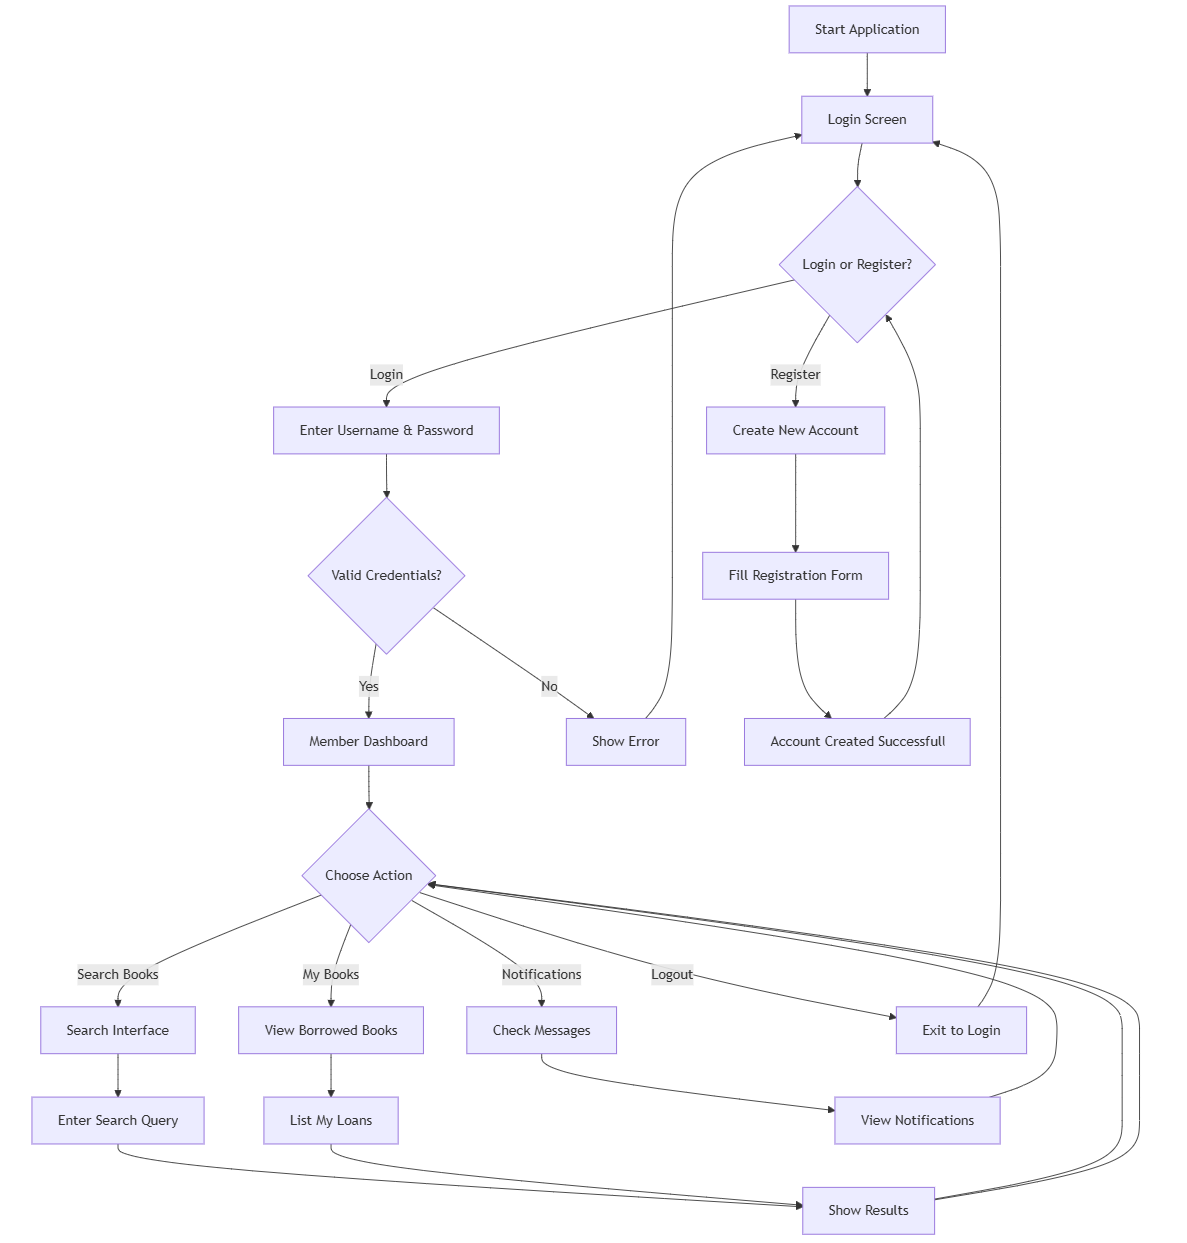
\includegraphics[width=\textwidth]{figures/member_workflow.png}
	\caption{Complete workflow diagram for library members.}
	\label{fig:member_workflow}
\end{figure}

\newpage

\subsection{Librarian Workflow Overview}
Librarians have access to administrative functions that enable them to manage the library's collection and oversee member activities. The librarian workflow includes adding new books to the catalog, updating book information, monitoring loan records, and managing member accounts. This administrative interface provides the tools necessary for effective library management. Figure \ref{fig:librarian_workflow} demonstrates the various administrative operations and decision points available to librarians.

\begin{figure}[H]
	\centering
	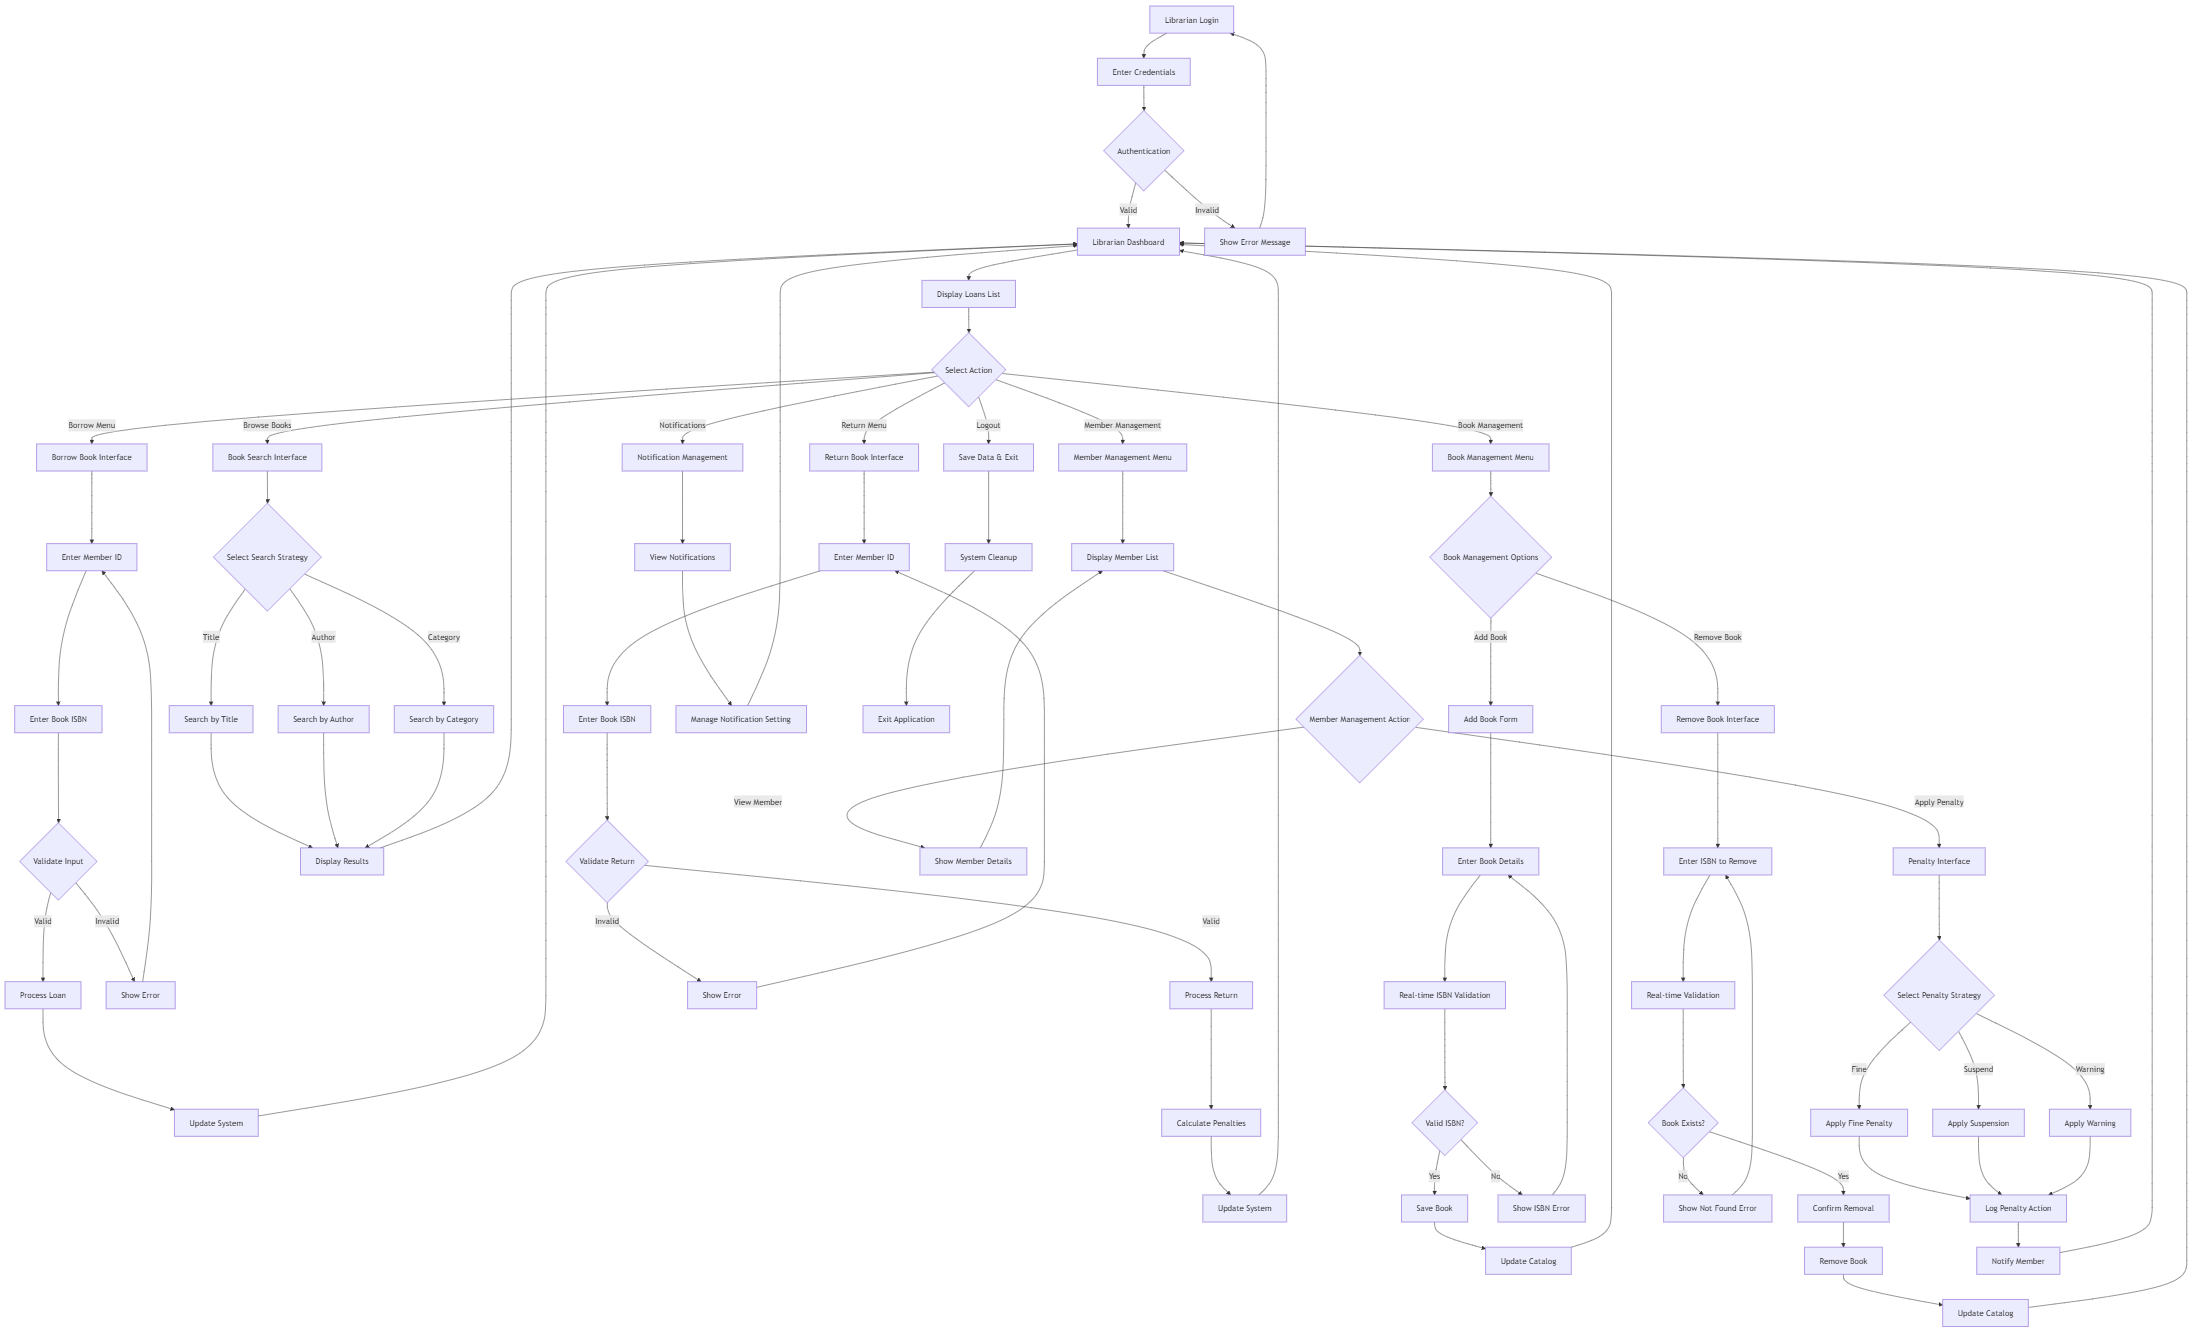
\includegraphics[width=\textwidth]{figures/librarian_workflow.png}
	\caption{Complete workflow diagram for library administrators.}
	\label{fig:librarian_workflow}
\end{figure}

\newpage

\subsection{Registering a New Member}
A new user interacts with the system to create a member account. The user selects the registration option from the main menu and provides the required credentials (username and password). The system then validates the input and creates a new member record, assigning a unique Member ID. The sequence of object interactions for this process is detailed in Figure \ref{fig:seq_register}.

\begin{figure}[H]
	\centering
	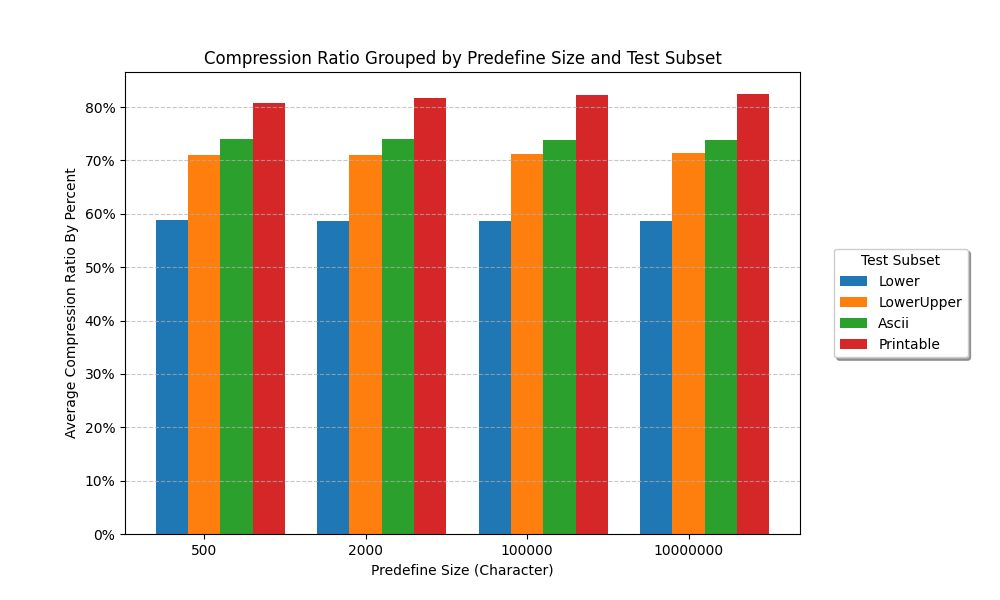
\includegraphics[width=\textwidth]{figures/sequence_register.png}
	\caption{Sequence Diagram for New Member Registration.}
	\label{fig:seq_register}
\end{figure}

\newpage

\subsection{Borrowing a Book}
A logged-in member can borrow a book from the library. The typical flow involves the member searching for a book and then selecting the "borrow" option, providing the book's ISBN. The system validates that the book is available, checks the member's borrowing eligibility, creates a new loan record, and finally updates the book's status. This workflow is visualized in Figure \ref{fig:seq_borrow}.

\begin{figure}[H]
	\centering
	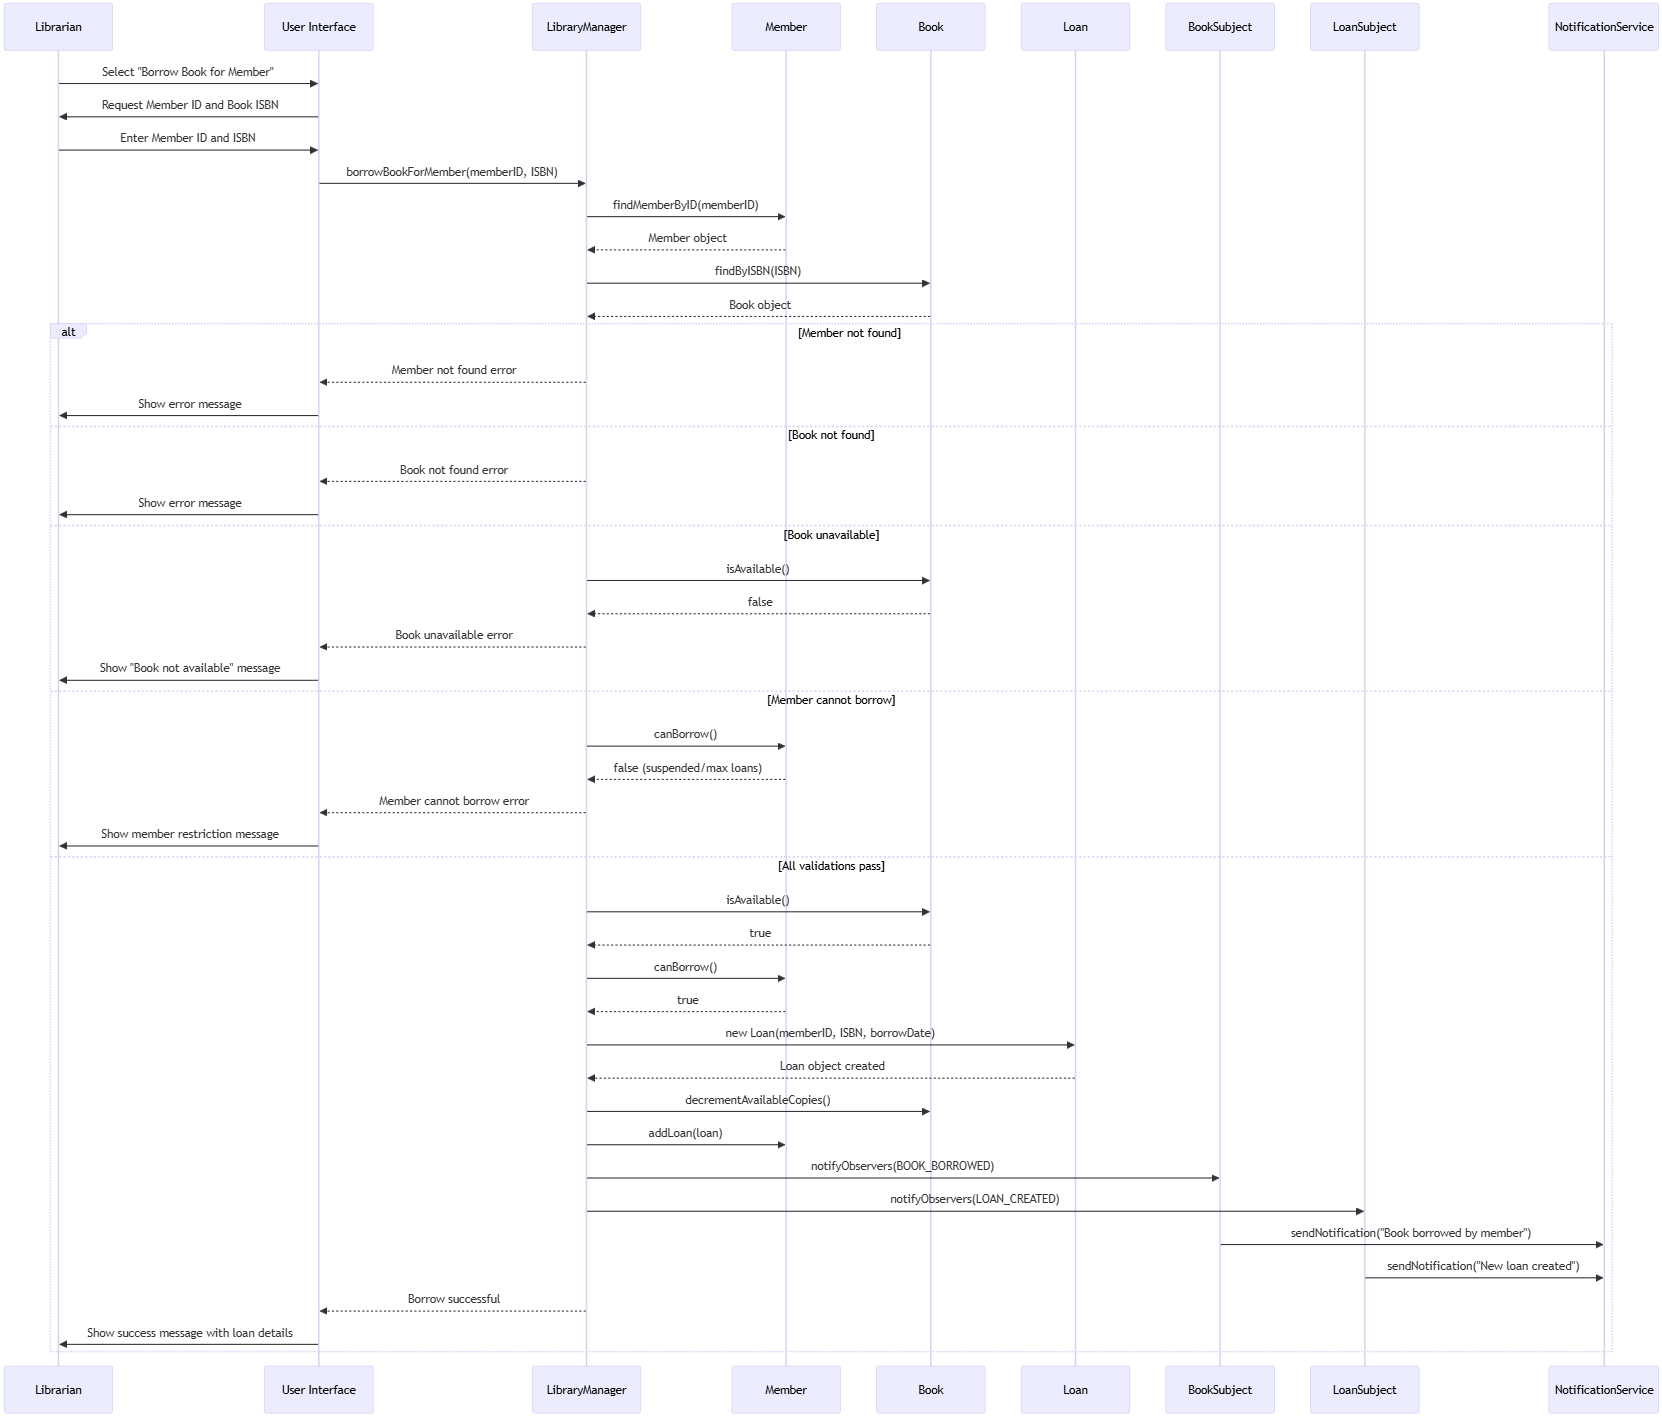
\includegraphics[width=\textwidth]{figures/sequence_borrow.png}
	\caption{Sequence Diagram for Borrowing a Book.}
	\label{fig:seq_borrow}
\end{figure}

\newpage

\subsection{Returning a Book}
When a member returns a book, they select the return option and provide the book's ISBN. The system finds the corresponding active loan record, updates its status to "returned," records the return date, and increments the number of available copies for that book. Figure \ref{fig:seq_return} illustrates the object interactions for this process.

\begin{figure}[H]
	\centering
	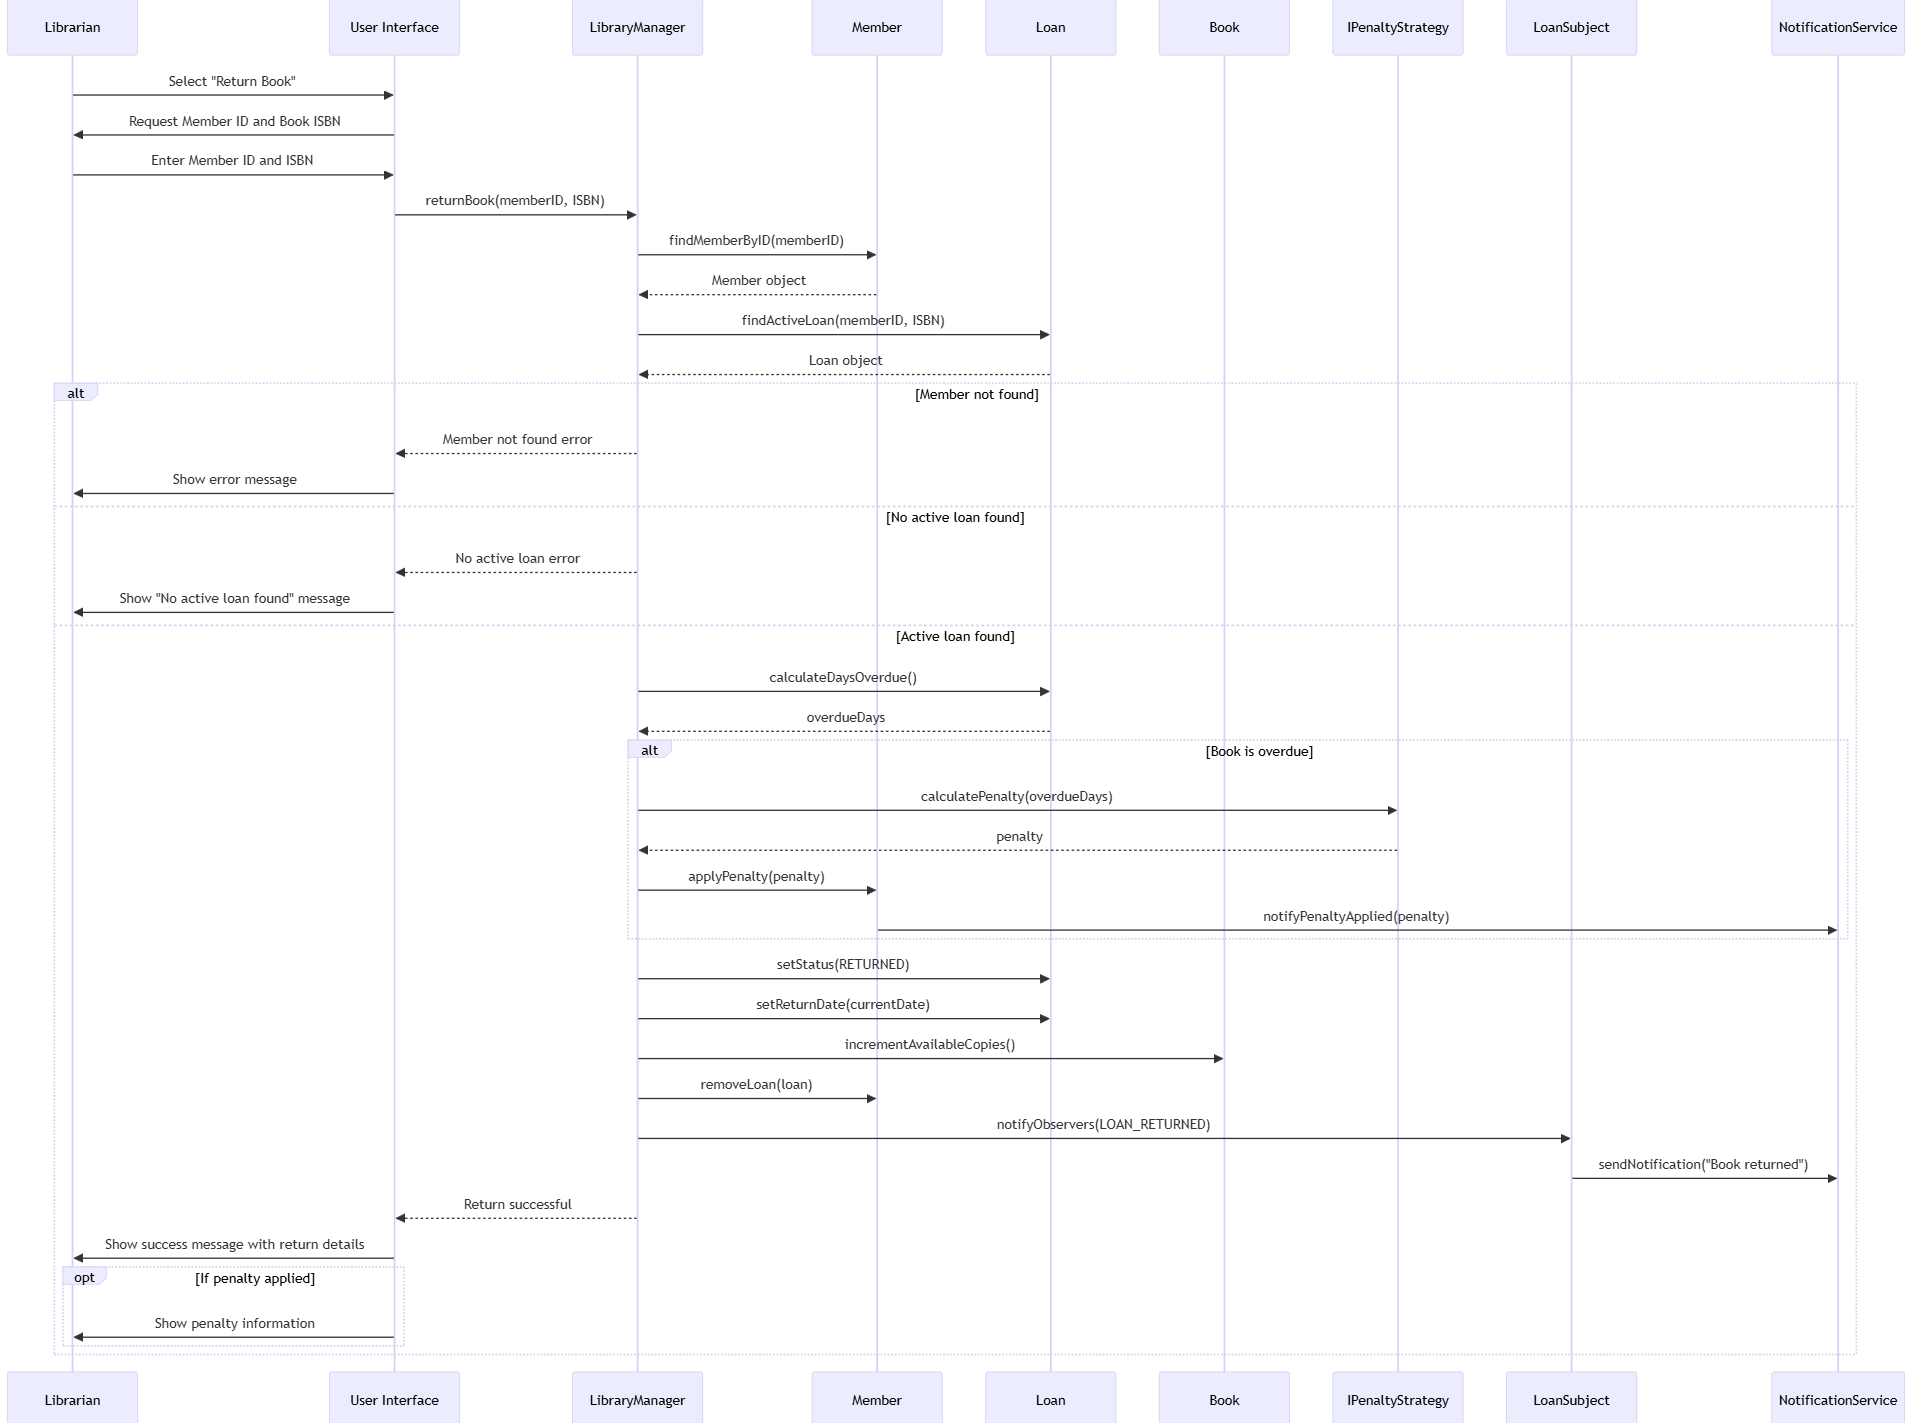
\includegraphics[width=\textwidth]{figures/sequence_return.png}
	\caption{Sequence Diagram for Returning a Book.}
	\label{fig:seq_return}
\end{figure}

\newpage

\subsection{User Interface Showcase}
The following screenshots provide a glimpse into the application's interactive console-based user interface, demonstrating its clarity and ease of use.

\begin{figure}[H]
	\centering
	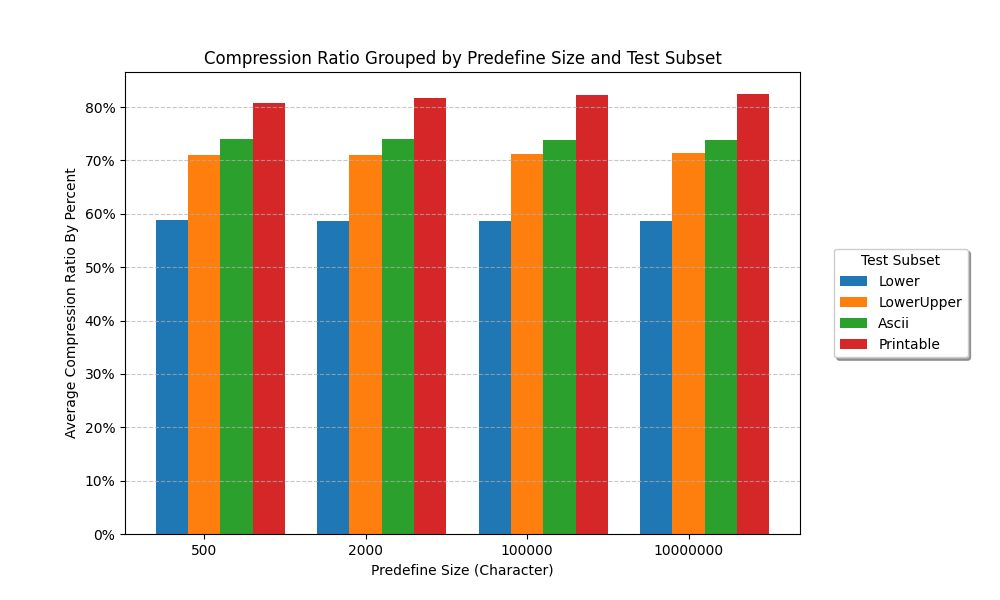
\includegraphics[width=0.9\textwidth]{figures/screenshot_main_menu.png}
	\caption{The main menu provides clear options for the user.}
	\label{fig:ss_main_menu}
\end{figure}

\begin{figure}[H]
	\centering
	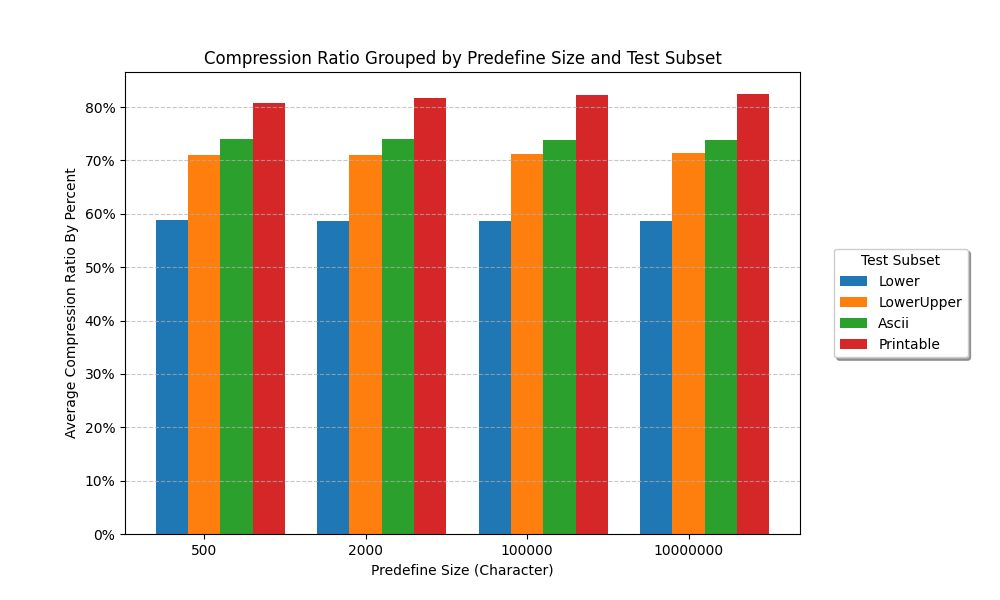
\includegraphics[width=0.9\textwidth]{figures/screenshot_search_result.png}
	\caption{An example of a book search result display.}
	\label{fig:ss_search}
\end{figure}